\documentclass[a4paper,11pt,twoside,openright]{article}

\usepackage[english]{babel}
\usepackage{color}
\usepackage{graphicx}
\usepackage[margin=3cm]{geometry}
\usepackage{hyperref}
\usepackage{epsfig,amsfonts}
\usepackage{xcolor,import}

\usepackage{subcaption}
\usepackage{amsmath,amssymb}  % Better maths support & more symbols
\usepackage{textcomp} % provide lots of new symbols\usepackage{natbib}
\usepackage[utf8]{inputenc}
\usepackage[T1]{fontenc}
\usepackage[french]{babel}
\usepackage{array,multirow,makecell}
\usepackage{gensymb}
\setcellgapes{1pt}
\makegapedcells
\newcolumntype{R}[1]{>{\raggedleft\arraybackslash }b{#1}}
\newcolumntype{L}[1]{>{\raggedright\arraybackslash }b{#1}}
\newcolumntype{C}[1]{>{\centering\arraybackslash }b{#1}}
\usepackage{geometry}
\geometry{hmargin=1.5cm,vmargin=2cm}

\pagestyle{plain}

\newcommand{\ud}[1]{\underline{#1}}
\newcommand{\e}[1]{\underline{e}_{#1}}
\newcommand{\lt}{\left}
\newcommand{\rt}{\right}
\DeclareMathOperator{\n}{\underline{n}}
\DeclareMathOperator{\ei}{\underline{e}_1}
\DeclareMathOperator{\et}{\underline{e}_2}
\DeclareMathOperator{\ex}{\underline{e}_x}
\DeclareMathOperator{\ey}{\underline{e}_y}
\DeclareMathOperator{\ez}{\underline{e}_z}
\DeclareMathOperator{\nin}{\underline{n}_{in}}
\DeclareMathOperator{\nout}{\underline{n}_{out}}
\DeclareMathOperator{\np}{\underline{n}_{P}}
\DeclareMathOperator{\bragg}{\theta_{bragg}}
\DeclareMathOperator{\DD}{\cos(\theta)^2 - \sin(\psi)^2}
\newcommand{\wdg}{\wedge}
\newcommand{\hypot}[1]{\textbf{\textcolor{green}{#1}}}


\begin{document}

\title{ToFu geometric tools \\ Take into account non-parallel crystal mesh}
\author{Adrien Da Ros}
\date{30/04/2021}
\maketitle

\tableofcontents
\newpage
\section{Problem details}
The definition into \textit{ToFu} geometrical tool of Bragg's crystals has been made to take into account geometrical, material and specific Bragg parameters. As we can see on Fig.\ref{fig:general_geom}, the crystal of curvature radius R has its center C on coordinates ($x_{c}$, $y_{c}$, $z_{c}$) in the Tokamak frame (O, $e_{x}$, $e_{y}$, $x_{z}$). \par

\begin{figure}[h]
    \centering
    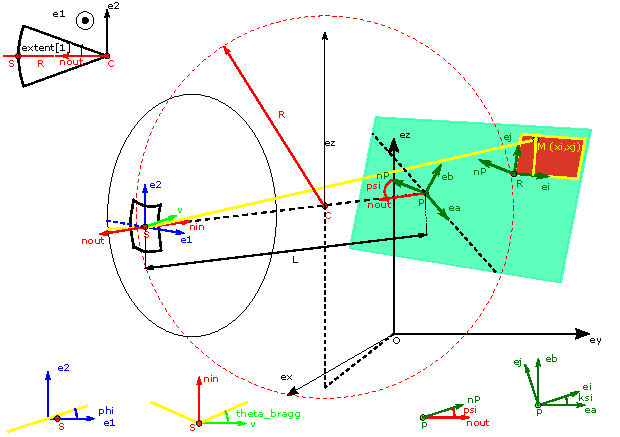
\includegraphics[width=0.8\textwidth]{SpectroX2D_Crystal.pdf}
    \caption{Definition of the generalized geometry}
    \label{fig:general_geom}
\end{figure}

This general description is assumed to be true at any time of the experiment. But there is one major issue that the current definition of the Bragg's crystals doesn't take into account, the non-parallelism of each crystal. As we can see on Fig.\ref{fig:non_para}, crystals are industrially made and sold with an index of confidence about the parallelism between the diopter and the crystal mesh. Because every crystal are not perfect, a maximum angle is furnished by the manufacturer, generally in arc-seconds. This defect causes a deviation of the normal vector $\nout$ shown in both Fig.\ref{fig:general_geom} and Fig.\ref{fig:non_para} (a deviation a is drawn).

\begin{figure}[h]
    \centering
    \includegraphics[width=1.\textwidth]{dessin.png}
    \caption{Definition of the non-parallelism between diopter $\overrightarrow{n_{in}}$ and mesh $\overrightarrow{n_{in}}^{'}$ unit vectors with a deviation a=$\alpha$ and d the distance in Angstroms between each layer.}
    \label{fig:non_para}
\end{figure}
\newpage
\section{Suggested trigonometrical solution}
The main issue due to this property of non-parallelism in each crystal can cause a splitting of the spectral lines.
In order to take into account this property, we propose first to define a orthogonal basis in spherical geometry based on the summit S of the crystal, as shown in Fig.\ref{fig:new_basis}.
Here, we took the same orthodirect basis as seen in Fig.\ref{fig:general_geom} ($\nout$, $\ei$, $\et$) where $\nout = -\nin$, the $\alpha$ angle represents the deviation's amplitude and the angle $\beta$ the new direction.

\begin{figure}[h]
    \centering
    \includegraphics[width=0.8\textwidth]{nouvelle_base_cristal_non_para.PNG}
    \caption{Definition of the the new basis 3D}
    \label{fig:new_basis}
\end{figure}
\newpage
Thanks to that, we can define easily now the new normal vector to the crystal mesh, which will be useful for few calculations.

$$
\lt\{
	\begin{array}{ll}
		\nout' & = cos(\alpha).\nout + sin(\alpha).(cos(\beta).\e1 + sin(\beta).\e2) \\
		\e1' & = \cos(\alpha)\lt(\cos(\beta).\e1 + \sin(\beta).\e2\rt) - \sin(\alpha).\nout\\
		\e2' & = \nout' \wdg \e1'\\
	\end{array}
\rt.
$$
$$
\e2' = \lt(cos(\alpha).\begin{vmatrix}
   \nout \\
   0 \\
   0
\end{vmatrix} + sin(\alpha).\lt(cos(\beta).\begin{vmatrix}
   0 \\
   \e1 \\
   0
\end{vmatrix} + sin(\beta).\begin{vmatrix}
   0 \\
   0 \\
   \e2
\end{vmatrix})\rt)\rt \wdg
\lt(\cos(\alpha)\lt(\cos(\beta).\begin{vmatrix}
   0 \\
   \e1 \\
   0
\end{vmatrix} + \sin(\beta).\begin{vmatrix}
   0 \\
   0 \\
   \e2
\end{vmatrix}\rt) - \sin(\alpha).\begin{vmatrix}
   \nout \\
   0 \\
   0
\end{vmatrix}\rt)$$
$$
\e2' = \begin{vmatrix}
   0 \\
   -\cos²(\alpha).\sin(\beta) + \sin²(\alpha).\sin(\beta) \\
   \cos²(\alpha).\cos(\beta) + \sin²(\alpha).\cos(\beta)
\end{vmatrix} 
= \begin{vmatrix}
   0 \\
   -\sin(\beta) \\
   \cos(\beta)
\end{vmatrix} = -\sin(\beta).\e1 + \cos(\beta).\e2
$$

So in the code, we shall propose the same notation according to Didier's work, ($\nout$, $\ei$, $\et$), in order to prevent some confusion between each set of parameters and to replace the original basis by the new one if the user does not assume perfect parallelism into its crystals. \par
The point is to let the user decide or not to give any parameter concerning the new basis and in this case the code will, if it's possible mathematically speaking, return all the parameters ($\nout$, $\ei$, $\et$, $\alpha$, $\beta$). If he doesn't, then a parallelism configuration will be assumed automatically and a warning notice will be shown in order to notice him about this point. Same thing about the missing of few parameters\par 
In order to compute the new unit vectors, the angles providing will be assumed as essential.









\end{document}
